\chapter{Results}
In this chapter, the results for our implementation and the baseline are presented for various configurations. Compression time and execution time for the operations are presented, along with the achieved compression factor. 

The datasets used for the evaluation are described in Section \ref{sec:datasets} and consist of: \emph{Sweden Buildings}, \textit{Sweden Roads}, \textit{Sweden All}, \textit{China Water}, and \textit{Admin Borders}. For intersection, a subset of \textit{Sweden All}, combined with \textit{China Water}, and \textit{Admin Borders} are used.

The computer used to benchmark was a MacBook Pro 2018 with a 2.9 GHz 6-Core Intel Core i9 processor and 32 GB 2400 MHz DDR4 RAM.

\section{Compression Factor \& Overhead}

In the following section, the compression factor is discussed with regard to various settings for the dataset and algorithm used. The compression factors are presented in Figure \ref{fig:compfactorres} and Table \ref{tab:compsize_tab}. When a limit is enforced on the number of deltas within a chunk to support faster random access, a maximum chunk length of 13 deltas is used. Furthermore, due to its widespread application in the industry, WKB is used as a reference for comparing the size of various configurations.
\\\\
The configurations used for the algorithm are described below and summarized in Table \ref{tab:comp_config}:

\begin{description}
     \item [WKB (Uncompressed)] Well-known binary to represent the shapes.
     
    \item [FPD] 64-bit floating-point delta encoding without support for efficient operations.

    \item [FPDE] The implementation referenced throughout the thesis. Consists of 32-bit integer decomposed coordinates and extensive metadata to allow efficient operations.
    
    \item [FPDE: Arbitrary Precision] FPDE using 64-bit floating-point delta encoding, i.e., the default encoding if not using 32-bit integer decomposed coordinates. The configuration has efficient support for operations.

    \item [FPDE: Entropy Encoding] FPDE with entropy encoding for the deltas. Each geometry is assigned the most size efficient entropy encoding method; either Huffman encoding, Golomb-Rice encoding or no entropy encoding.

    \item [FPDE: Size Optimized] FPDE using 32-bit integer decomposed coordinates, without any extra metadata for the operations. No limit on the number of deltas per chunk and entropy encoding is applied without the size overhead, which disables random access.

    \item [WKB: gzip] WKB, followed by \textit{gzip} compression.
    
    \item [WKB: bzip2] WKB, followed by \textit{bzip2} compression.
\end{description}

\begin{table}[h]
\centering
{\setlength{\extrarowheight}{5pt}%
\resizebox{\textwidth}{!}{%
\begin{tabular}{|l|l|l|l|l|}
\hline
\textbf{\begin{tabular}[c]{@{}l@{}}Compression \\ Method\end{tabular}} & \textbf{\begin{tabular}[c]{@{}l@{}}Floating-Point\\ Encoding Scheme\end{tabular}} & \textbf{\begin{tabular}[c]{@{}l@{}}Support for \\ Operations\end{tabular}} & \textbf{\begin{tabular}[c]{@{}l@{}}Max Chunk\\ Length\end{tabular}} & \textbf{\begin{tabular}[c]{@{}l@{}}Entropy \\Encoding\end{tabular}} \\ \hline
WKB (Uncompressed)                                                     & 64-bit IEEE 754                                                                   & \ding{51}                                                                        & -                                                                      & \ding{53}                                                                            \\ \hline
FPD                                                         & 64-bit IEEE 754                                                                   & \ding{53}                                                                         & \ding{53}                                                                     & \ding{53}                                                                            \\ \hline
FPDE: Arbitrary Precision                                               & 64-bit IEEE 754                                                                   & \ding{51}                                                                        & \ding{51}                                                                     & \ding{53}                                                                            \\ \hline
FPDE                                                                   & \begin{tabular}[c]{@{}l@{}}32-bit integer \\ decomposed coordinates\end{tabular}    & \ding{51}                                                                        & \ding{51}                                                                    & \ding{53}                                                                            \\ \hline
FPDE: Entropy Encoding                                                 & \begin{tabular}[c]{@{}l@{}}32-bit integer  \\ decomposed coordinates\end{tabular}    & \ding{51}                                                                        & \ding{51}                                                                    & \ding{51}                                                                           \\ \hline
FPDE: Size Optimized                                                   & \begin{tabular}[c]{@{}l@{}}32-bit integer \\ decomposed coordinates\end{tabular}    & \ding{53}                                                                        & \ding{53}                                                                     & \ding{51}                                                                           \\ \hline
WKB: gzip                                                              & 64-bit IEEE 754                                                                   & \ding{53}                                                                         & -                                                                      & \ding{51}                                                                            \\ \hline
WKB: bzip2                                                             & 64-bit IEEE 754                                                                   & \ding{53}                                                                         & -                                                                      & \ding{51}                                                                            \\ \hline
\end{tabular}}}
\caption{The methods used for compression with their respective configurations summarized.}
\label{tab:comp_config}
\end{table}

\begin{figure}[htbp]
    \centering
    \includesvg[width=12.0cm]{images/comp_factor.svg}
    \caption{Compression factor for various configurations. 30 000 random samples from each dataset were used. Average of all shape's factors. WKB is used as the uncompressed representation and the factor is thus in relation to WKB.}
    \label{fig:compfactorres}
\end{figure}


\begin{table}[htbp]
\centering
\caption{Compression factor and ratio (\%) when calculated over all samples, i.e., the combined size of all shapes in WKB representation divided by the combined compressed size.}
%\begin{adjustwidth}{-1cm}{}
\resizebox{\textwidth}{!}{%
\begin{tabular}[h]{l|ccccccccc}
\toprule
Dataset & WKB & FPD & Arbitrary & FPDE & Entropy & Size Opt & WKB: gzip & WKB: bzip2 \\
\midrule 
Sweden Buildings & 1.0 (100) & 1.85 (54) & 0.88 (113) & 1.82 (54) & 1.8 (55) & 4.45 (22) & 0.75 (133) & 1.07 (93) \\
Sweden Roads & 1.0 (100) & 1.57 (63) & 0.95 (105) & 2.11 (47) & 2.11 (47) & 4.22 (23) & 0.79 (126) & 1.05 (95) \\
Sweden All & 1.0 (100) & 1.65 (60) & 1.04 (96) & 2.34 (42) & 2.39 (41) & 4.64 (21) & 0.92 (108) & 1.2 (83) \\
China Water & 1.0 (100) & 1.67 (59) & 1.2 (83) & 2.78 (35) & 2.85 (35) & 4.73 (21) & 1.09 (91) & 1.31 (76) \\
Admin Borders & 1.0 (100) & 1.39 (71) & 1.07 (93) & 2.21 (45) & 2.64 (37) & 4.22 (23) & 1.18 (84) & 1.3 (76) \\
\midrule
Average & 1.0 (100) & 1.62 (61) & 1.03 (97) & 2.25 (44) & 2.56 (39) & 4.45 (22) & 0.95 (105) & 1.18 (84) \\ 
\bottomrule
\end{tabular}}
%\end{adjustwidth}
\label{tab:compsize_tab}
\end{table}





Figure \ref{fig:compfactorres} and Table \ref{tab:compsize_tab} show that the compression factor is affected by the compression algorithm used and the attributes of the datasets. The order of the algorithms with the highest compression factors remains consistent across the various datasets, where the general-purpose algorithms perform the worst, and FPDE with disabled partial decompression performs the best. As shown in the same figure, some configurations generally perform better on certain datasets than others. In the following section, a comparison between the results for the different algorithm variations is presented, followed by an analysis of the effects that the attributes of the datasets have on the compression ratio.

\subsubsection{Algorithm Comparison}
According to Table \ref{tab:compsize_tab}, the order of the average compression performance is: \textit{WKB: gzip}, \textit{WKB}, \textit{FPDE: Arbitrary Precision}, \textit{WKB: bzip2}, \textit{FPD}, \textit{FPDE}, \textit{FPDE: Entropy Encoding}, followed by \textit{FPDE: Size Optimized}. The general-purpose algorithms are expected to perform the worst, as they do not exploit domain-specific structures and are based on general ideas. When comparing the performance between the FPDE configurations, they seem to be ordered by the format of the floating-point coordinates, the overhead of supporting optimized operations, and whether entropy encoding is utilized or not. 

\begin{figure}[htbp]
    \centering
    \includesvg[width=15cm]{images/overhead_distr.svg}
    \caption{The total size distribution within average geometries from the datasets using FPDE. \textit{Chunk BBs} is the overhead of the bounding boxes of the chunks, required by the optimized intersection operation. A maximum chunk length of 13 deltas and no entropy encoding was applied. 100 000 random samples were used.}
    \label{fig:overheaddistrb}
\end{figure}

The distribution of various components in FPDE is visualized in Figure \ref{fig:overheaddistrb}, where it can be seen that the overhead of the operations in FPDE occupies a significant amount of space. This is the main reason why \textit{FPDE: Size Optimal} yields superior compression compared to \textit{FPDE}, along with the utilization of entropy encoding. Additionally, since \textit{FPDE: Size Optimal} does not require additional overhead to support operations with entropy encoded deltas, the format gains the full effect of entropy encoding, shown in Table \ref{tab:entropyDeltas}. On the contrary, when comparing \textit{FPDE: Entropy Encoding} to \textit{FPDE} in Table \ref{tab:compsize_tab}, it is discovered that the extra overhead, which allows the former to perform operations with entropy encoded deltas, offsets the gains of the entropy encoding.

Another observation is the effect of using different formats for representing the geometry coordinates, where algorithms that utilize 32-bit integer decomposed coordinates outperform those using 64-bit IEEE 754 floating-point coordinates. However, while the effect is self-evident, using the former comes at the cost of its coordinate precision constraint of 7 decimals, as outlined in Section \ref{32-bit}. Additionally, it is essential to note that for configurations that use 32-bit  coordinates, the compression factor is directly increased, due to the halving of the bit representation from 64 to 32 bits.  Thus, in those cases, if operation speed is lacking and the compression factor is close to the effect of just changing the floating-point representation, it would be unnecessary to utilize the integrated operation support. Instead, it might be beneficial to store the geometries directly using the 32-bit format without additional compression, and run the operations directly to avoid the extra decompression overhead. Therefore, to representatively compare the effect caused by the induction of operability on the compression ratio, the algorithm configurations that use the same coordinate format should be compared, such as \emph{FPD} versus \emph{FPDE: Arbitrary} and \emph{FPDE: Size Optimized} versus \emph{FPDE: Entropy Encoding}. As evident by Figure \ref{fig:overheaddistrb}, the operation overhead represents a significant portion of the data, resulting in a decreased compression ratio. However, it is worth noting that the overhead varies greatly on a per-shape basis, and that the overhead of the chunk bounding boxes likely can be significantly reduced in future work by, for example, using a quadtree.

\subsubsection{Influence of Dataset Attributes}
As evident by Figure \ref{fig:overheaddistrb}, the distribution between various components in FPDE varies heavily between the datasets. Alongside the \textit{$\mathrel\#$ Vertices} column in Table \ref{tab:chunks}, it is apparent that there is a correlation between the number of vertices in the geometries and the proportion of deltas in its compressed form. As deltas are the essence of compression, they contribute to an increased compression factor. The reason for the increase in proportion of deltas is that with more complex shapes, the overhead of the global bounding box data diminishes in relation to the coordinate data. Additionally, as seen in Table \ref{tab:chunks}, the average number of vertices in each chunk is higher for datasets with a higher vertex count, causing more deltas in relation to coordinates represented in full. 

\begin{table}[htbp]
\centering
\caption{Chunking statistics based on an average of 100 000 random samples with a maximum chunk size of 13 deltas.} 


\label{tab:dataset_stats_chunking}
%\begin{adjustwidth}{-1.3cm}{}
\resizebox{\textwidth}{!}{%

\begin{tabular}{@{\extracolsep{4pt}}lcccccc}
\toprule   
 {} & {} & {} & {} & \multicolumn{3}{c}{$\mathrel\#$ Vertices in Chunks}\\
 \cmidrule{5-7}
Dataset & $\mathrel\#$ Vertices & Delta Bit Size & $\mathrel\#$ Chunks & Average & Standard Deviation & Median \\ 
\midrule
Sweden Buildings & 6.3 & 12.3 & 1.0 & 5.0 & 0.1 & 5.0 \\ 
Sweden Roads & 12.7 & 13.7 & 1.6 & 6.5 & 1.0 & 6.7 \\
Sweden All & 16.3 & 13.2 & 1.9 & 6.4 & 0.8 & 6.5 \\ 
China Water & 63 & 14.1 & 5.8 & 9.7 & 2.4 & 10.2 \\ 
Admin Borders & 278 & 20.2 & 30.4 & 9.8 & 4.2 & 11.1   \\ 
\bottomrule
\end{tabular}
}
%\end{adjustwidth}
\label{tab:chunks}
\end{table}

The compression factor is also affected by the efficiency of the deltas, specifically how many bits each delta occupies. The average number for this across the different datasets is outlined in the \textit{Delta Bit Size} column in Table \ref{tab:chunks}. This observation clarifies why, although \textit{Admin Borders} have a higher fraction of deltas compared to \textit{China Water} and \textit{Sweden All}, the average compression factor is lower.

The variance for the compression ratio between different shapes also differs between the datasets. For example, as shown in Figure \ref{fig:compfactorres}, while the geometries in the \textit{Sweden Buildings} dataset seem to achieve a consistent compression factor, it varies greatly in the \textit{Sweden Roads} dataset. The reason for the variance is the homogeneity of shapes within the datasets, where buildings tend to be more similiar than roads.






% Fyra separata grafer, en för varje dataset. Består av:
% - WKB storlek, GZIPPad WKB, FPD, FPDE med alla operationer 7 decimaler, FPDE med alla operationer floating point (första iden), FPDE med alla operationer + entropy 7 dec, FPDE utan operationer med entropy 7 dec

%Eventuellt visa compression ratio med t-box plots:
% - Fpd
% - Fpde (int32) med operationerna
% - Fpde (int32) med operationer + entropy
% - Fpde (int32) entropy (auto) -random access (ingen bbox eller intersection)+ intcoord
% - Fpde (float) med operationer
% - Wkb
% - Wkb med gzip
% - Wkb med bzip2



% Ha tabell med byte size (inte filens utan själva binstring), + för de där uppe. Rader som alg, kolumn för dataset, även Wkb.Comp factor i parentes



\section{Execution Time for Operations}
\subsection{All Operations}
\label{sec:exec_time}
To achieve a fair comparison of the timing of the operations, with as little influence by implementation details as possible, both the baseline and FPDE use the 64-bit IEEE 754 floating-point representation with no entropy encoding of the deltas. These configurations are previously referred to as \textit{FPD} and \textit{FPDE: Arbitrary Precision}, respectively. However, the results are expected to generalize to 32-bit integer decomposed coordinates with entropy encoded deltas when used by both the baseline and FPDE, as the decompression stage will be more complex and result in an increased execution time of the decompression stage. The gains of partial decompression are greater when the compression stage of the operation accounts for a larger fraction of the complete operation compared to the actual operation; since then, decreasing the number of decompression operations has a greater impact relative to the baseline. Note that, when evaluating partial decompression, it does not make sense to compare with a baseline that uses a different compression scheme (for instance \textit{FPD} versus \textit{FPDE: Entropy Encoded}), as it is likely that the comparison will be influenced to a greater extent by the effectiveness of the compression scheme, as opposed to the use of partial decompression.

\begin{figure}[htbp]
    \centering
    \includesvg[width=14cm]{images/operation_exec_time.svg}

    \caption{Mean relative execution time (per geometry) in relation to the baseline (dotted black line) for different operations using FPDE. }
    \label{fig:op_time}
\end{figure}

The execution time of FPDE is presented in relative proportion to the execution time of the baseline. When evaluating, 100 000 random samples were taken from both the \textit{Sweden All} and \textit{China Water} datasets, and 5 000 samples were taken from the \textit{Admin Borders} dataset. For the binary operations, an equal number of sample pairs were used.

\begin{table}[htbp]
\centering
\resizebox{\textwidth}{!}{%
\begin{tabular}{lc|cccccc}
\hline
Dataset & Algorithm & Compress & Decompress & Bounding Box & Add Vertex & Is Intersection & Intersection \\
\hline
\multirow{2}{*}{Sweden All} & FPDE & 301 & 104 & 3 & 27 & 8 & 19 \\
 & Baseline & 299 & 103 & 87 & 574 & 121 & 131 \\
\hline
\multirow{2}{*}{China Water} & FPDE & 642 & 234 & 3 & 35 & 8 & 18 \\
 & Baseline & 562 & 218 & 200 & 962 & 381 & 394 \\
\hline
\multirow{2}{*}{Admin Borders} & FPDE & 3168 & 1236 & 3 & 61 & 9 & 24 \\
 & Baseline & 2866 & 1205 & 1138 & 4237 & 2394 & 2349 \\
\hline
\end{tabular}%
}
\caption{Table of absolute execution time (µs) for different datasets and operations when using the baseline and FPDE.}
\label{tab:comparison}
\end{table}

Examining Figure \ref{fig:op_time} and Table \ref{tab:comparison}, it appears that except for \textit{compress} and \textit{decompress}, performing operations on random samples using the extended format outperforms the baseline setting. The speed of  \textit{compress} and \textit{decompress} is entirely determined by the amount of input data, and for FPDE, the additional overhead to enable support for the operations leads to a relative execution time above 100\%. As depicted in Figure \ref{fig:overheaddistrb}, the overhead fraction of the datasets varies, and conclusively the compress and decompress operations will have relative execution times deviating between the datasets.


For the \textit{Bounding Box} operation, the constant cost of extracting a fixed number of bits from a given offset in FPDE is clearly more efficient than decompressing the entire geometry and performing the bounding box calculation. The reason why the relative speed differs between the datasets is due to the decompression stage of the baseline. For geometry datasets that contain complex shapes, such as \textit{Admin Borders}, decompression takes longer than for \textit{Sweden All} and \textit{China Water}, which have a lower average vertex count per shape.

For \textit{Add Vertex}, the reasoning is similar; modifying a fixed number of bits at a given offset is faster than complete decompression. Similarly to the \textit{Bounding Box} operation, the relative execution time varies between the datasets due to the difference in the decompression time of the baseline.

Moreover, for the binary operations \textit{Is Intersection} and \textit{Intersection}, as outlined in Section \ref{sec:intersection}, the initial stage of both algorithms checks for a shared bounding box between the shapes. If such a common bounding box is absent, no intersection can occur, and the operations return. For a random pair of geometries in a large dataset, the likelihood of intersection is very low, and for the great majority of cases a common bounding box will not exist. In these cases, the execution terminates quickly and, conclusively, the mean of the relative execution time for the binary operations in Figure \ref{fig:op_time} does not fully reflect the situations where the pair of shapes intersect. Section \ref{sec:res_intersection} includes a more extensive analysis of how the binary operations perform in different contexts and geometry complexities.




\subsection{Intersection}
\label{sec:intersection_results}
In this section, additional intersection cases in terms of context and vertex count of the involved shapes are examined in more detail. As mentioned in Section \ref{sec:exec_time}, the performance of both intersection operations is heavily dependent on the geometries' context and sizes, and therefore it is not sufficient to look at a global mean value when making conclusions about the execution time. 

When two geometries' bounding boxes overlap, we differentiate between the cases where one geometry is fully contained in the other (\textit{Contained}), two geometries bounding boxes overlap but there is no intersection (\textit{Disjoint}), and lastly, the geometries have crossing line segments (\textit{Crossing}). Furthermore, the size category refers to the number of vertices in the shape. Large geometries have at least 100 vertices, medium have between 50 and 100, and small have less than 50. Large and small geometries are also referred to as \textit{complex} and \textit{simple} shapes, respectively. For the results below, 100 000 geometry pairs from each of the \textit{Admin Borders}, \textit{China Water} and \textit{Sweden All} datasets were used.

The subsequent reasoning is in the context of \textit{Intersection}, but the same logic can be applied to \textit{Is Intersection}.

\begin{figure}[htbp]
    \centering
        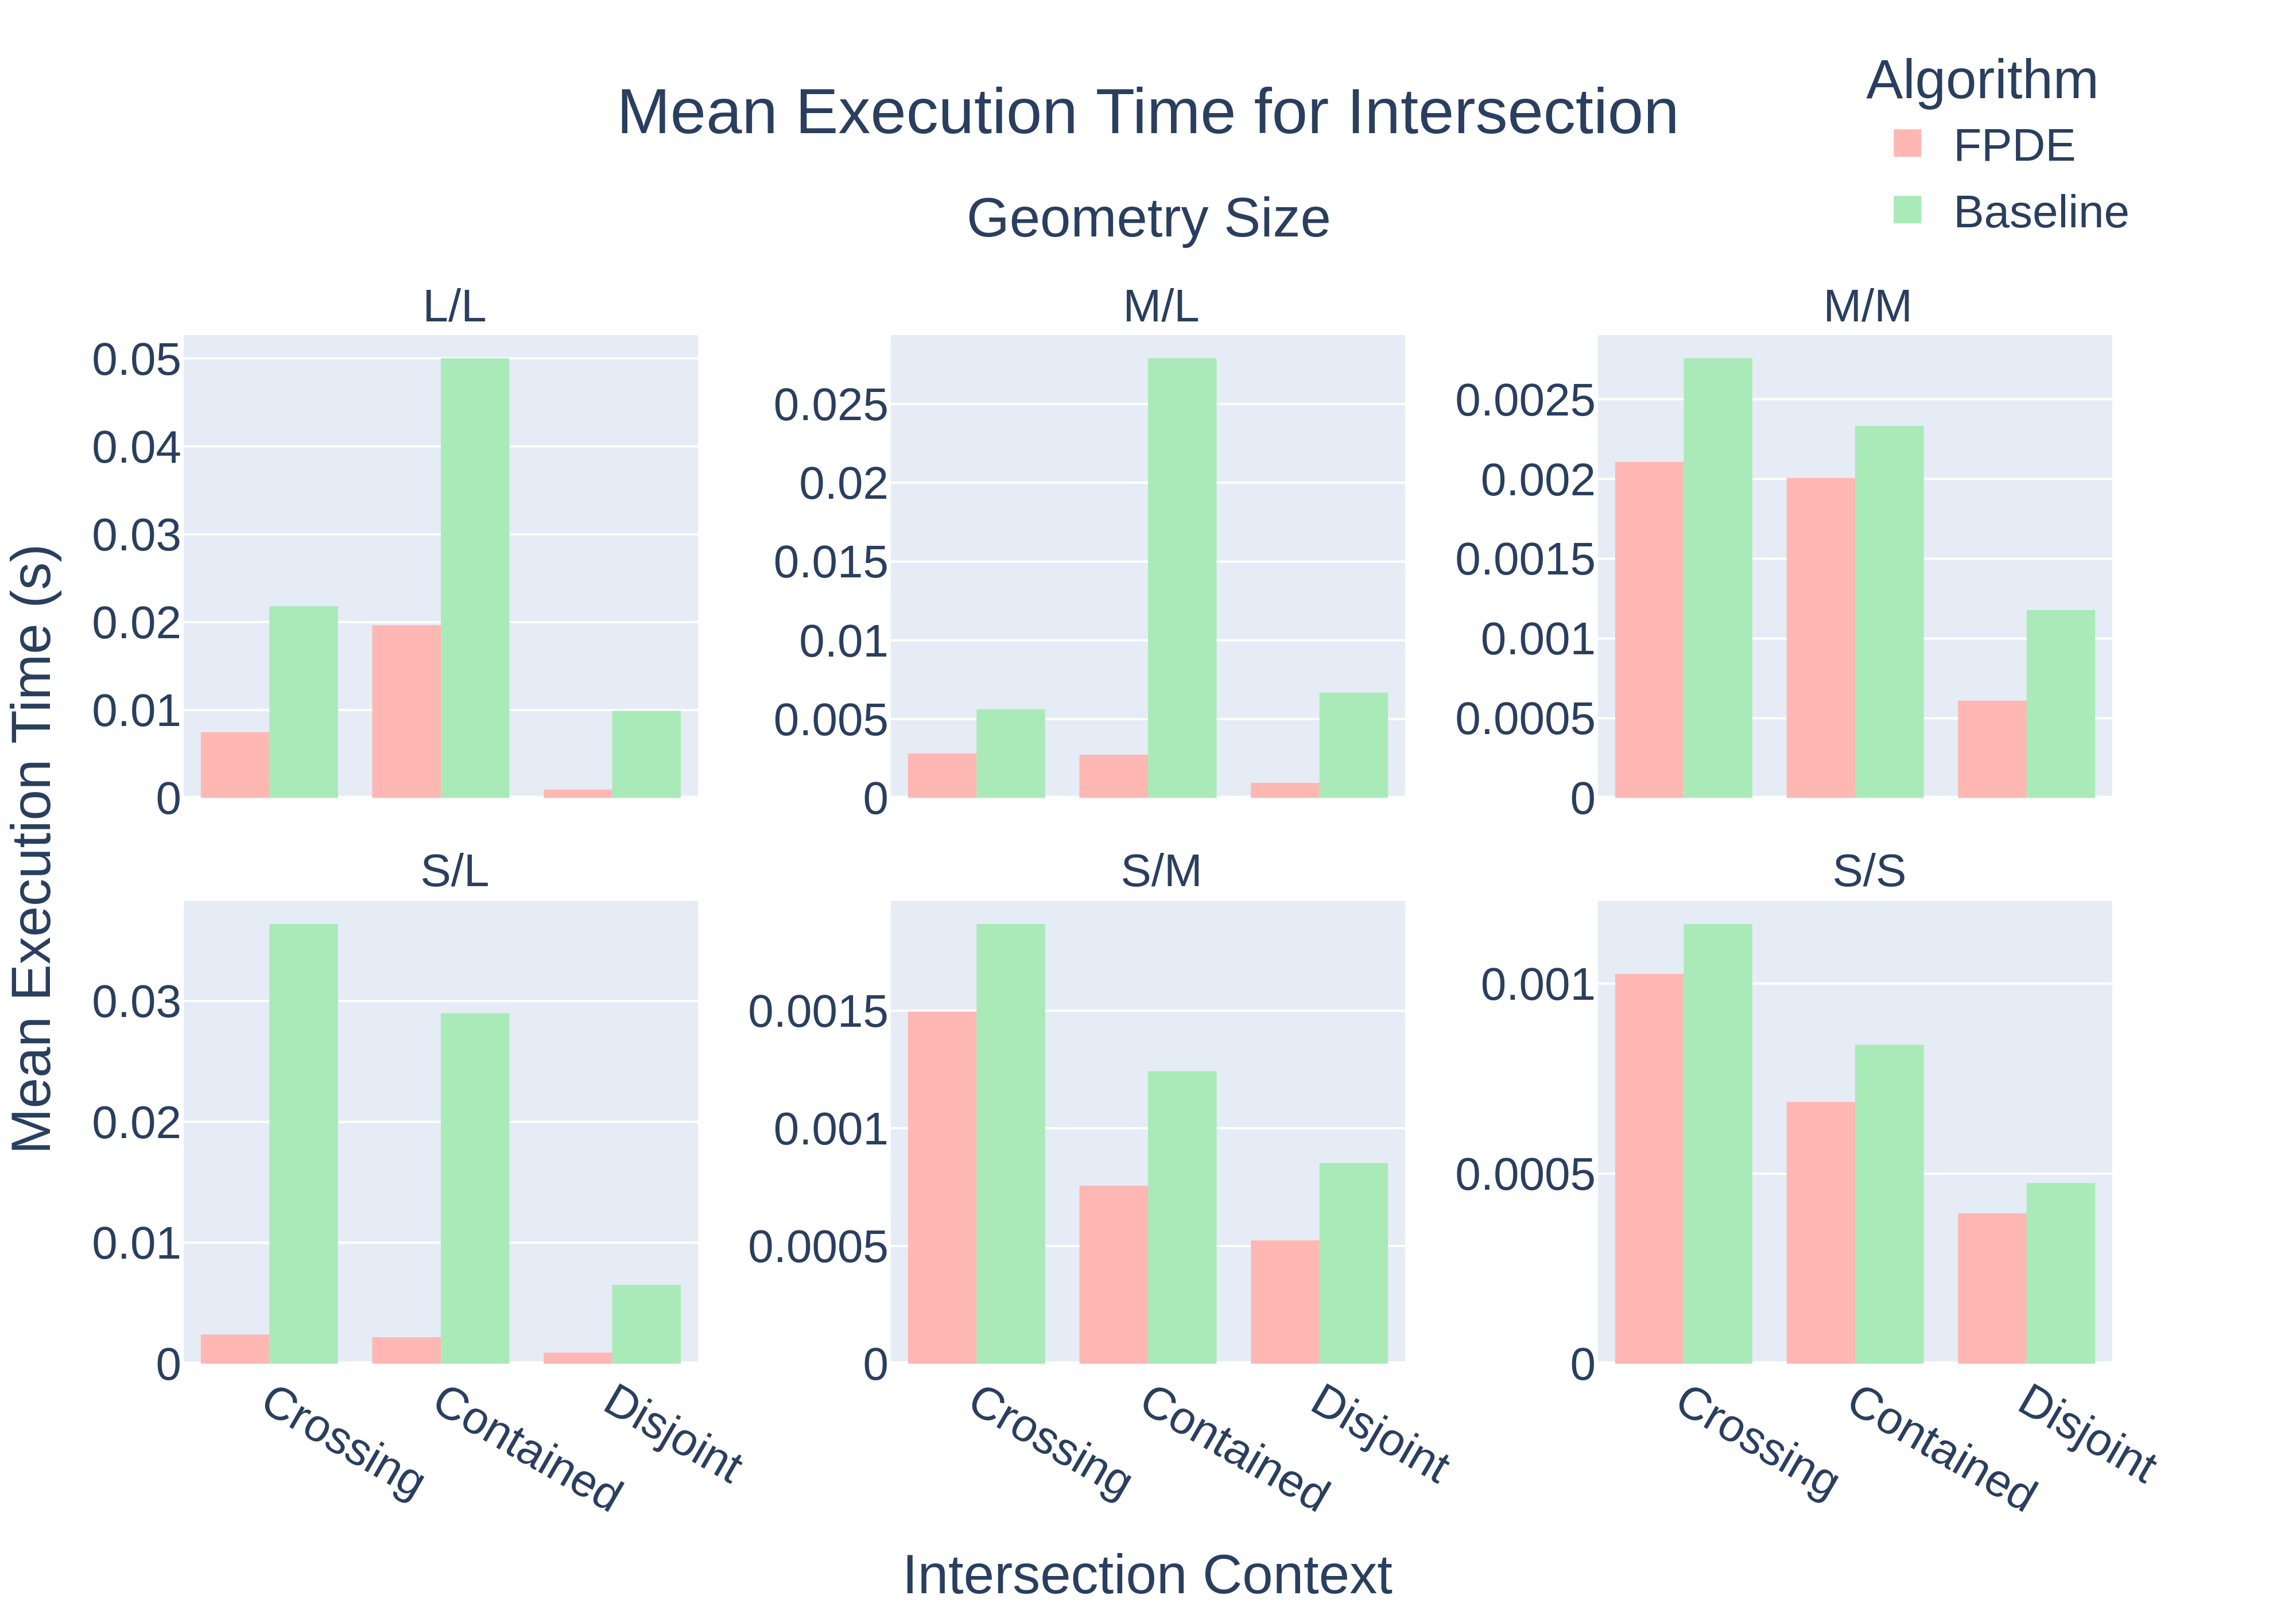
\includegraphics[width=14.5cm]{images/intersection_fpde_vs_baseline.png}

        \caption{Average execution time for FPDE for different contexts and geometry sizes. }
        \label{img:meanIntersection}
\end{figure}

\begin{figure}[htbp]
    \centering
    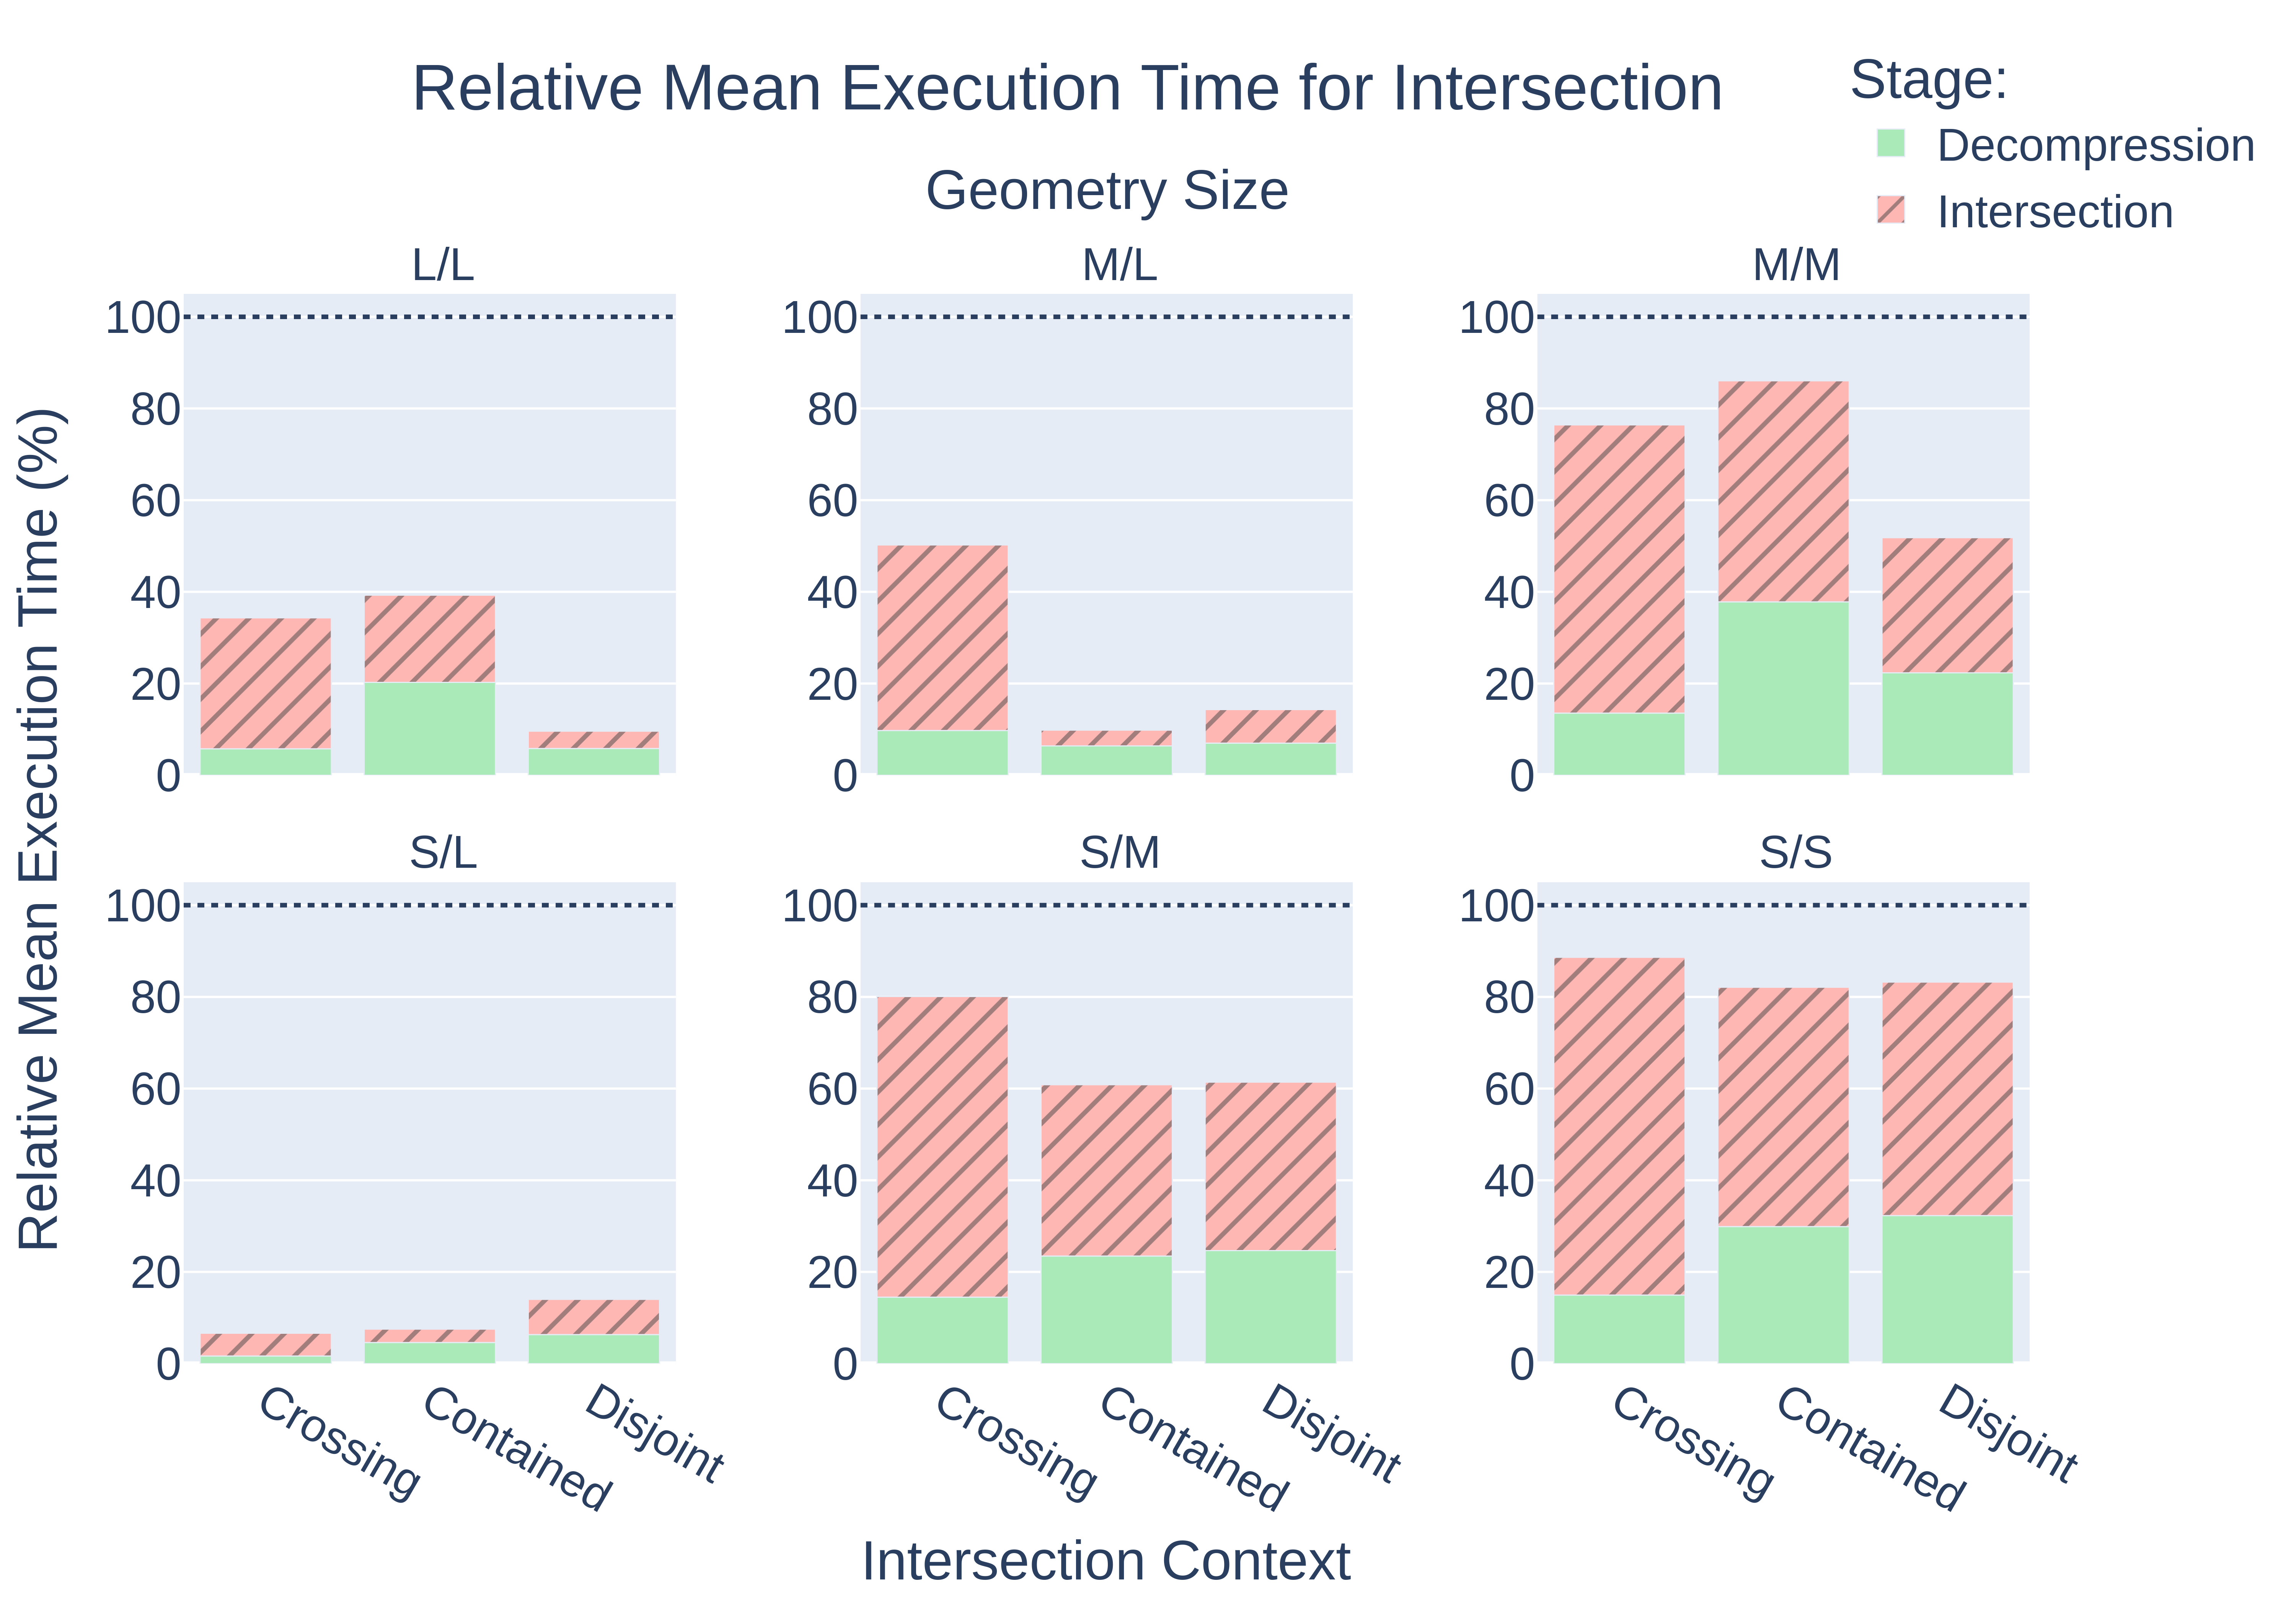
\includegraphics[width=14.5cm]{images/relative_mean_exec_time.png}
    \caption{Fractions for the relative execution time of the decompression and the intersection algorithm stage for FPDE. }
    \label{img:Intersection_exec_time}
\end{figure}

\subsubsection{Number of Vertices in Geometries}
Figure \ref{img:meanIntersection} and \ref{img:Intersection_exec_time} show that the gain of using FPDE for intersection is more significant in scenarios involving complex geometries. This is because complex geometries consist of more chunks, which potentially enables the filtering step in the algorithm to be more fine-grained. In contrast, if a geometry only contains one single chunk, the filtering step has no flexibility in selecting only a subset of the vertices. This reasoning is further supported by Figure \ref{fig:chunks_unfold} showing that on average, calculating the intersection of two simple geometries involves decompressing almost all available chunks, while only a tiny fraction is unfolded for complex geometries.

\begin{figure}[htbp]
    \centering
    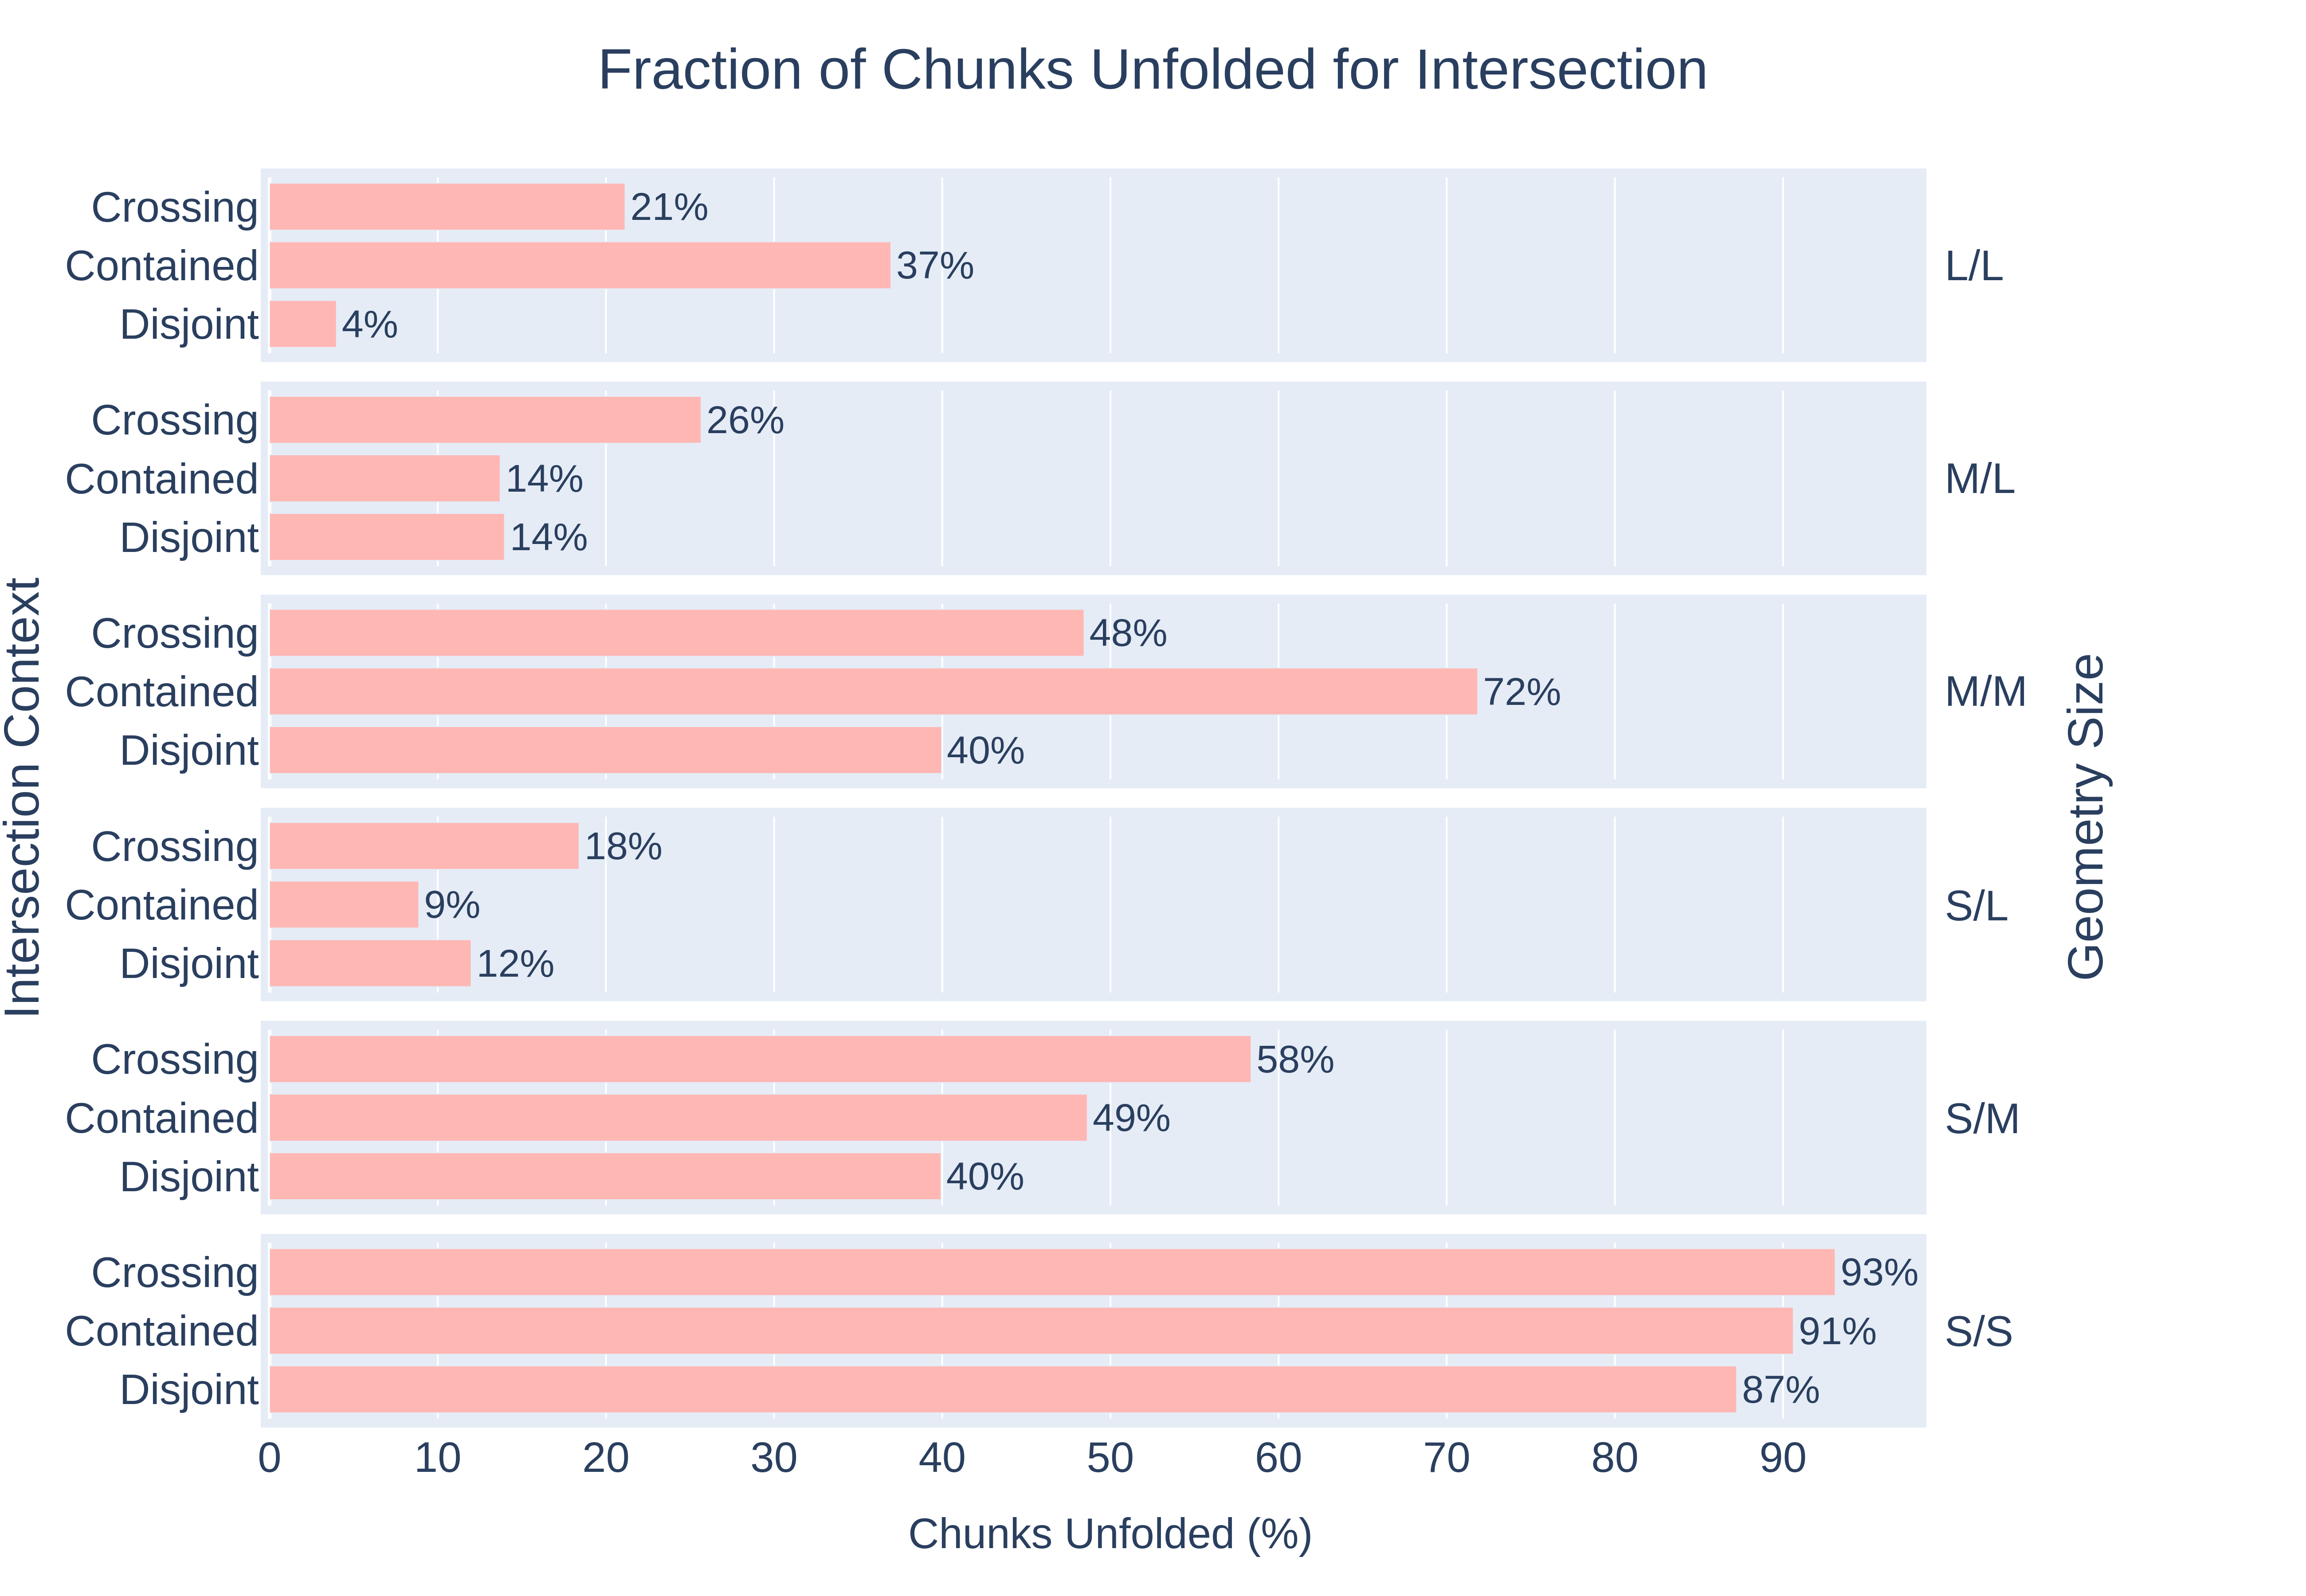
\includegraphics[width=15cm]{images/fraction_of_chunks_unfolded}
    \caption{Fraction of chunks partially decompressed grouped by context and dataset.}
    \label{fig:chunks_unfold}
\end{figure}

\subsubsection{Intersection Context}
The execution time of the intersection operation also depends on the context of the geometries. For example, in the \textit{Contained} case, the performance gain of using FPDE depends on the complexity of the contained geometry. Figure \ref{img:meanIntersection} shows that when a simple or medium-sized geometry is contained within a complex geometry, FPDE significantly outperforms the baseline. This is because FPDE only has to decompress the smaller inner geometry and a tiny fraction of the complex outer geometry, when performing the testing for \emph{contains}, described in Section \ref{sec:pointinshape}.

In contrast, when the geometries' size categories are equal, the relative execution time and the fraction of chunks unfolded are relatively high, as shown in Figure \ref{img:Intersection_exec_time} and \ref{fig:chunks_unfold}. In these circumstances, it is likely that the shapes are tightly arranged, which causes many of the chunk bounding boxes to overlap, resulting in unnecessary decompression for some of the outer geometry's chunks. 

When averaging the relative execution time for FPDE in contexts with two large geometries in Table \ref{tab:partial_decomp_tab}, FPDE achieves an execution time faster by a factor of 3.6 relative to the baseline, which uses full decompression.


\begin{table}[htbp]
\centering
\resizebox{8.5cm}{!}{
\begin{tabular}{|m{2.2cm}|m{1.3cm}|>{\centering\arraybackslash}m{1.8cm}|>{\centering\arraybackslash}m{1.4cm}|>{\centering\arraybackslash}m{1.4cm}|}  % Adjust column widths and center the percentage columns
\hline
\textbf{Context} & \textbf{Size} & \textbf{FPDE RME (\%)} & \textbf{FPDE PD (\%)} & \textbf{Baseline PD (\%)} \\
\hline
Crossing & L/L & 34 & 17 & 36 \\
& M/L & 50 & 19 & 41 \\
& M/M & 76 & 18 & 30 \\
& S/L & 7 & 25 & 52 \\
& S/M & 80 & 18 & 30 \\
& S/S & 89 & 17 & 23 \\
\hline
Contained & L/L & 39 & 52 & 60 \\
& M/L & 10 & 65 & 82 \\
& M/M & 86 & 44 & 54 \\
& S/L & 8 & 61 & 81 \\
& S/M & 61 & 39 & 52 \\
& S/S & 82 & 36 & 42 \\
\hline
Disjoint & L/L & 10 & 61 & 85 \\
& M/L & 14 & 49 & 77 \\
& M/M & 52 & 43 & 66 \\
& S/L & 14 & 45 & 75 \\
& S/M & 61 & 40 & 59 \\
& S/S & 83 & 39 & 48 \\
\hline
\end{tabular}}
\caption{Table with the relative difference of the mean execution time for FPDE in relation to the baseline, along with the percentage of time spent on partial decompression versus the intersection operation for FPDE and the baseline.}
\label{tab:partial_decomp_tab}
\end{table}

\subsubsection{Decompression \& Actual Intersection Operation Relationship}
In Table \ref{tab:partial_decomp_tab}, the relative execution time of FPDE relative to the baseline is presented, together with the corresponding fractions of time dedicated to the decompression or intersection stage. Figure \ref{img:Intersection_exec_time} is a complementary visualization to the table focusing on FPDE. The table shows that the baseline spends more relative time of its execution on decompression in general. Furthermore, it can be inferred that a low relative execution time for FPDE is closely correlated with the proportion of decompression in the total execution. For instance, intersection contexts with low values for the relative mean execution time are coupled with a high ratio of time spent on partial decompression.





\newpage
\label{sec:res_intersection}
\subsection{Intersection: Deltas Size–Time Trade-Off}
\label{sec:chunking}
The variable partitioning into chunks impacts both the compression ratio and the execution time of operations utilizing partial decompression for random access, explained in Section \ref{Random_access}. 
As FPDE has the ability to set a maximum number of deltas allowed per chunk, the partitioning of the chunks can vary depending on the parameter value. 

\begin{figure}[htbp]
    \centering
        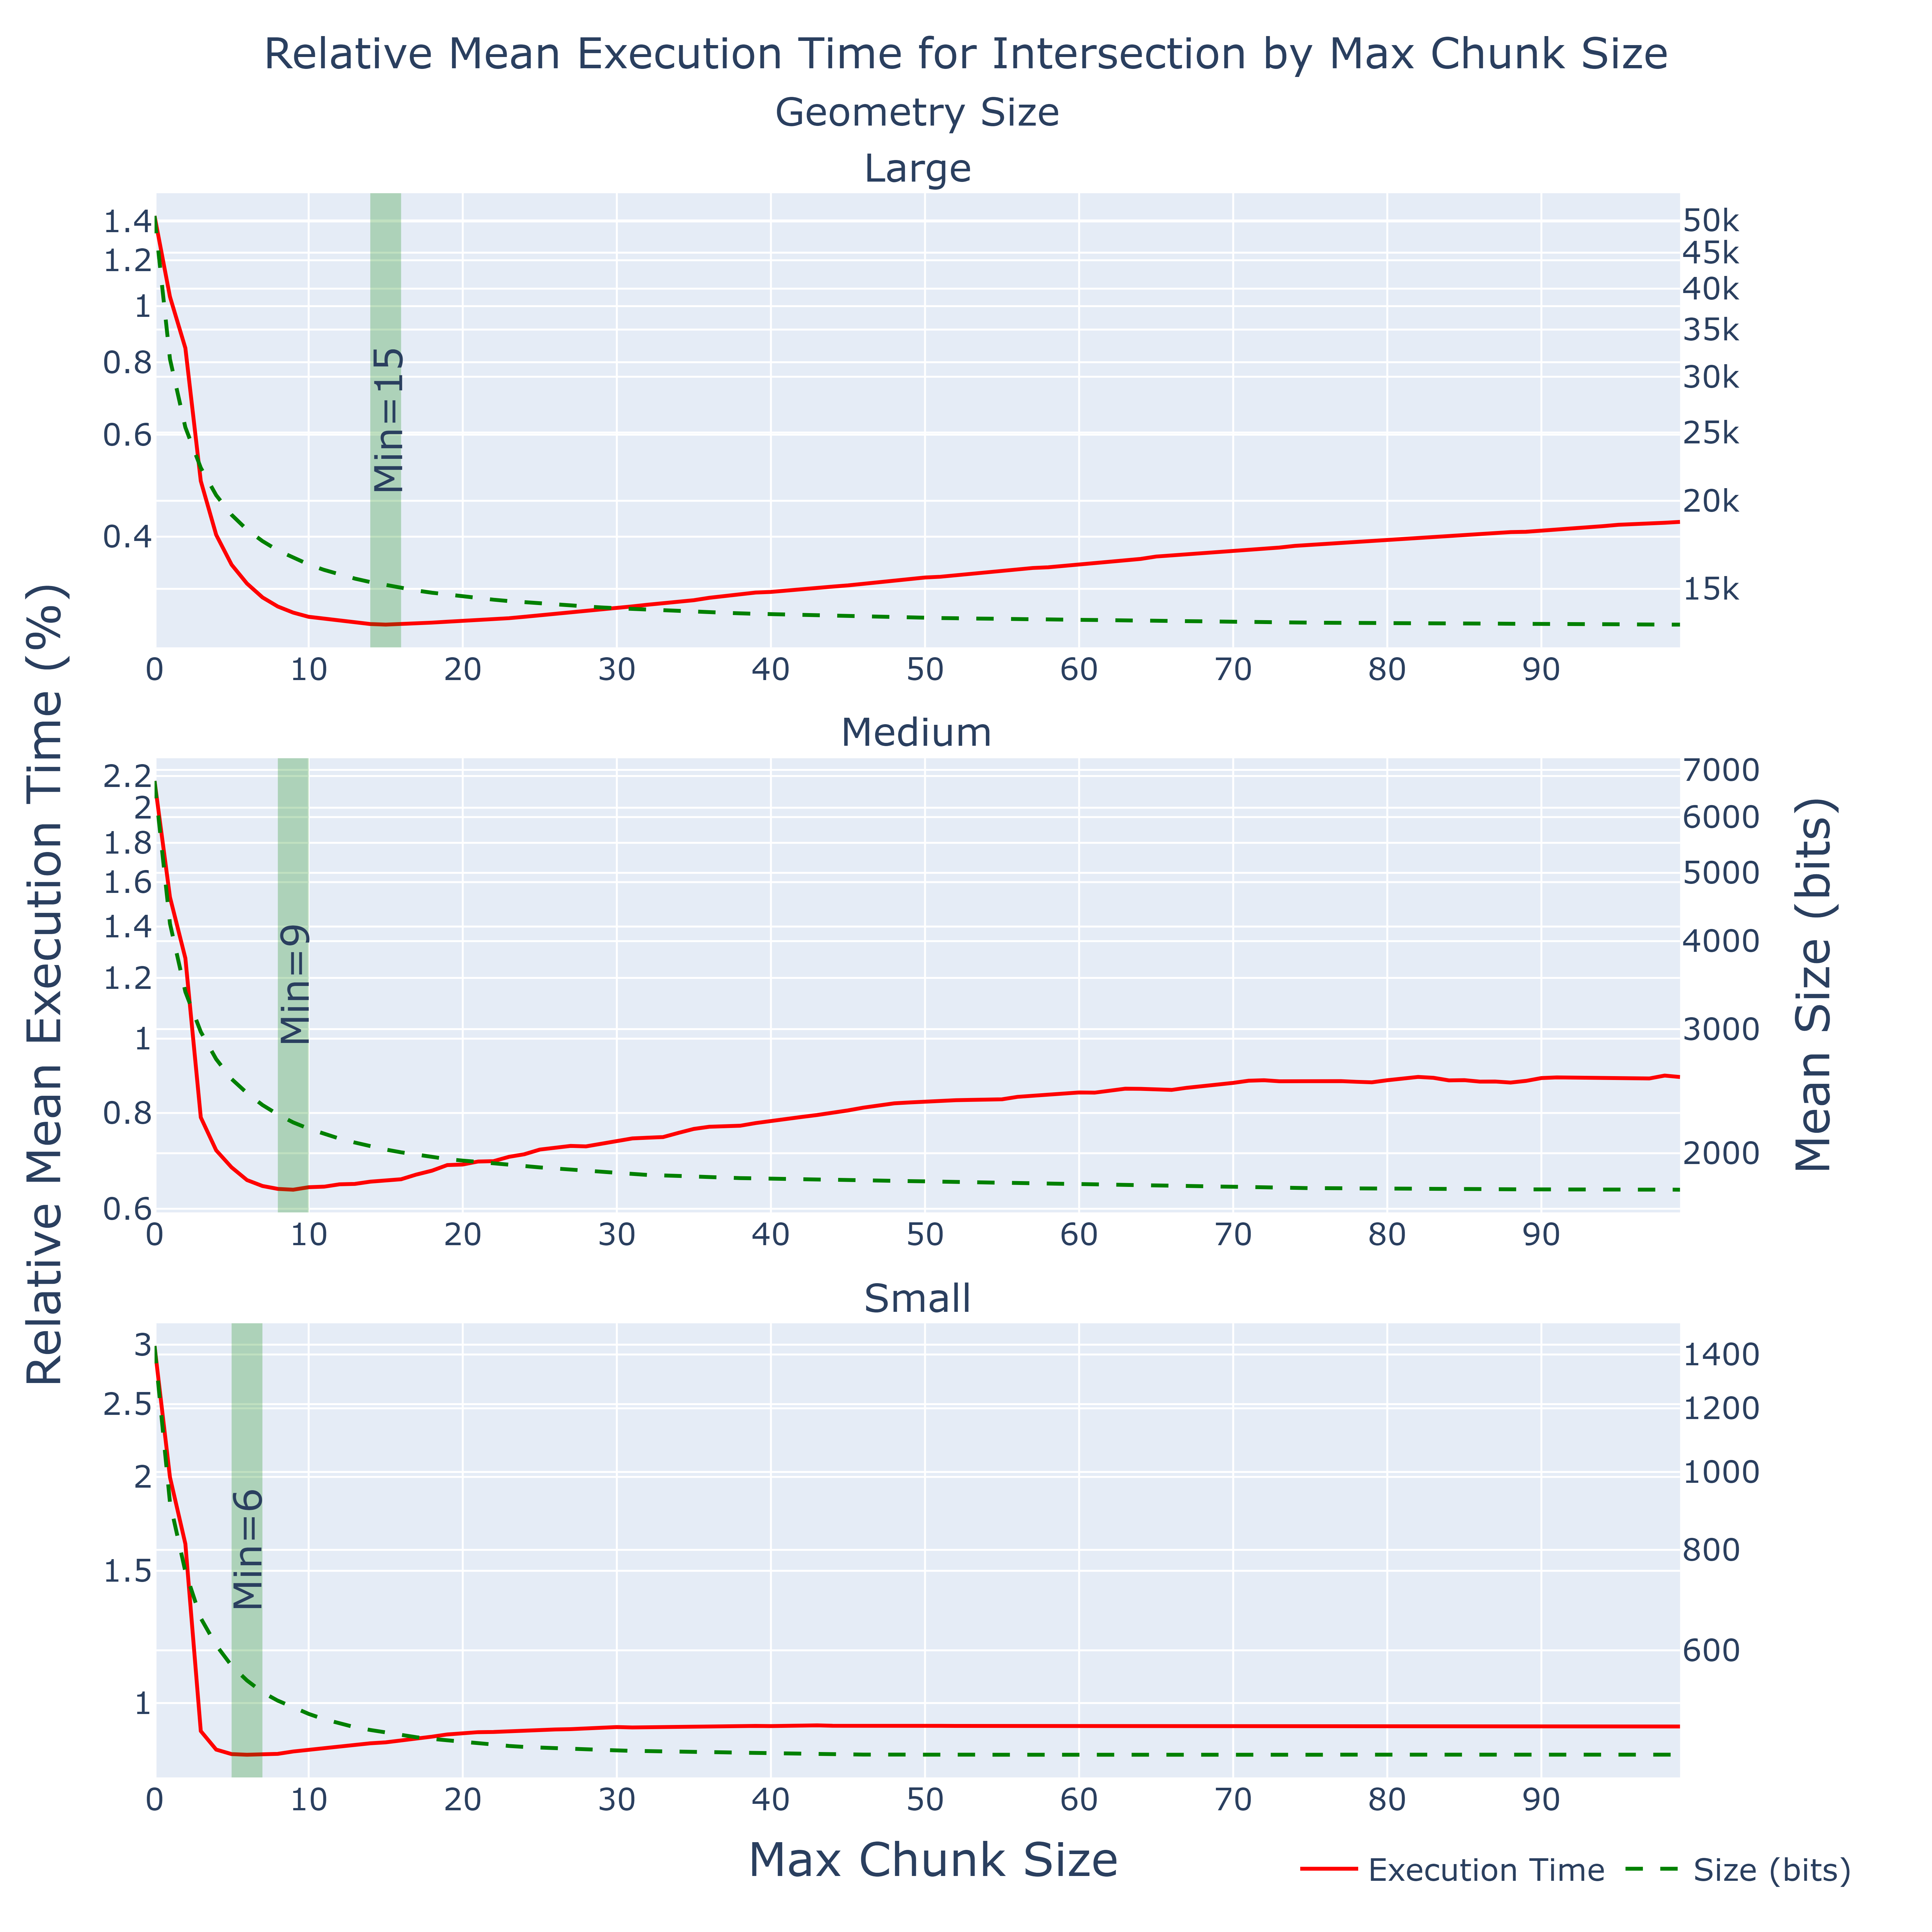
\includegraphics[width=15.5cm]{images/chunk_max_size.png}
    \caption{The left axis (red line) shows the relative mean execution time between FPDE and the baseline with a moving average window of three to compensate for noise, and the left axis (green line) shows the average bit size by the max chunk size parameter.}
    \label{img:delta_max_chunk_perf}
\end{figure}

\subsubsection{Impact on Compression Ratio}
Figure \ref{img:delta_max_chunk_perf} shows how the resulting bit size varies with the maximum chunk size. Increasing the parameter results in a higher average compression factor due to fewer chunk breaks, requiring less coordinates to be represented in full, whereas a small parameter value decreases the compressibility and introduces additional overhead.

The ratio between the number of full coordinates and deltas, if assuming no automatic chunking, can be described with the expression \(r(d) = \frac{1}{d + 1}\), where \(d\) is the maximum number of deltas in a chunk. As the formula and Figure \ref{img:delta_max_chunk_perf} suggests, the ratio decays rapidly, and the effect of the parameter is most significant at lower values.

When setting the parameter to zero and using integrated operability with the default floating-point format, i.e., disabling 32-bit integer decomposed coordinates, the size becomes larger than WKB. This is because setting the value to zero essentially disables delta encoding and introduces additional overhead since each coordinate also includes a chunk header.

On the contrary, when setting an unlimited chunk size, a new chunk is only created when a delta does not fit within the shape's delta bit-length. For homogeneous shapes, the number of chunks is therefore lower since the automatic splitting of the chunks occurs less frequently.

\subsubsection{Impact on Execution Time of Intersection}
As observed in the same figure, the relative mean execution time for intersection also depends on the selection of the maximum number of deltas in each chunk. For intersection queries, the parameter affects two stages, jumping to the correct chunk start and the chunks' decompression time. When increasing the max chunk size, the chunks become fewer and so does the number of jumps required to reach a chunk. On the contrary, when the parameter increases, the chunks also get bigger, and the decompression of each chunk takes longer.

The maximum chunk size also affects the spatial filtering of relevant chunks in the operation. As depicted in Figure \ref{fig:intworld}, intersection queries only extract the relevant chunks through pairwise comparison of the chunks' bounding boxes. For larger chunks, the bounding box will be bigger and, if chunks are too large, irrelevant segments are frequently decompressed due to being in relevant chunks.

In Figure \ref{img:delta_max_chunk_perf}, it also seems that datasets with complex shapes have a slower decay in relative mean execution time with an increased chunk size, compared to datasets with simpler shapes. This is likely due to the fact that complex shapes are able to utilize more chunks, since they have more vertices. The reason for the asymptotic stabilization in execution time when greatly increasing the max chunk size is likely due to deltas overflowing, forcing new chunks even though the chunk max size is not reached.

\subsubsection{Size-Time Trade-Off}
Combining the results above, it is apparent that setting the parameter of maximum chunk size has a large effect on both the size and performance. For the evaluation of the thesis, the value resulting in the highest speed has been chosen. But in a real-world setting, the value can be tweaked to prioritize either size or speed.





% Eventuellt hand picka några fall för att kunna göra djupare analys:
% Strand med ex. en väg som korsar
% Två shapes som är typ helt överlappande


% I bild ovan, mergea datasets, lägg till grå bar (komplement), fixa caps

\section{Entropy Encoding of Deltas}
%Entropy Metrics}
% Huffman, Golomb, Huff Golomb, Huffman Stripped , https://docs.python.org/3/library/bz2.html för burrows wheeler
% Presentera resultat från notebooken, inte huvuddelen av exjobbet så håll kort
For the entropy encoding and analysis of the deltas \textit{32-bit integer decomposed coordinates}, as described in Section \ref{32-bit}, were used to encode the coordinates. All deltas within the datasets presented in Section \ref{sec:datasets} were combined and used for the entropy encoding and evaluation. Note that since the delta values are zigzag encoded integer decomposed coordinates, the values represent the doubled distances between consecutive vertices with alternating signedness. For example, the floating-point decoding of zigzagged values $2$, $3$, and $10000$ is $+ {\color{gray}0.000000}1$, $- {\color{gray}0.000000}1$, and $+ {\color{gray}0.000}5000$.

\begin{figure}[H]
    \centering
    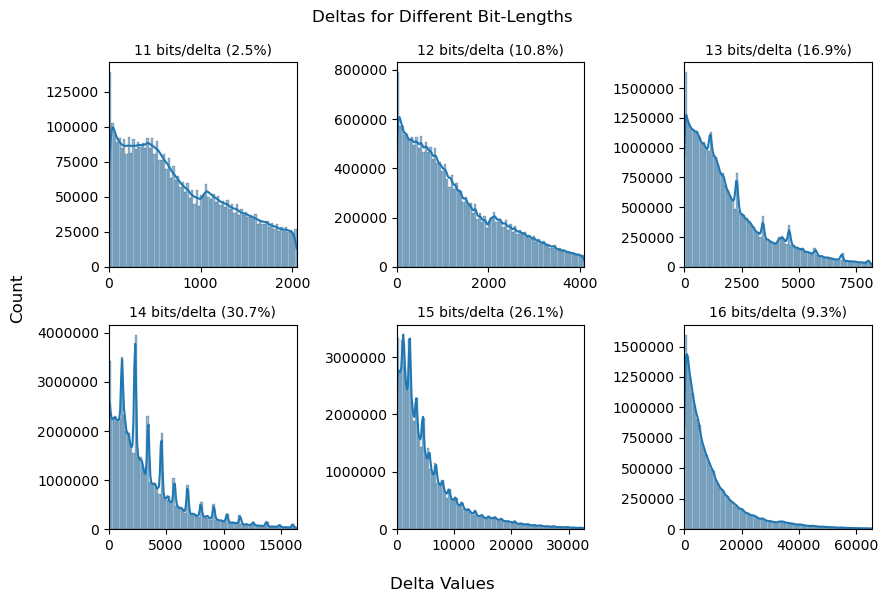
\includegraphics[width=15cm]{images/delta_distrb.png}
    \caption{Frequency distribution of the zigzag encoded delta values interpreted as unsigned integers for the combined datasets. Only the delta bit-lengths accounting for more than 1\% of the combined datasets are visible. 80 bins are used.}
    \label{fig:deltadistrb}
\end{figure}


When analyzing the deltas, it can be concluded that the distribution of values is not uniform. As seen in Figure \ref{fig:deltadistrb}, the values are heavily concentrated around zero, with some spikes in specific values. It is also evident that the decay follows a distribution that closely resembles a geometric distribution, where the slope of the distribution increases for larger delta bit-lengths. According to Figure \ref{fig:deltadistrb}, it seems that the spikes are not present for large delta bit-lengths, but manual analysis concludes that the absence in the graph is instead a result of the binning used when plotting and that the spikes are persistent.

After manually examining the combined frequencies for all bit-lengths, it can be concluded that the most common delta value is 0, followed by $\pm 0.0001145$ and additional seemingly random small values. 0 accounts for 1.5\% and $+ 0.0001145$ for 0.97\% of the values. The spikes then decrease rapidly, where the ten most common values amount to 6\%, and the ten to hundred most common values amount to 8\% of all values.

Zero being the most common value is expected since when a shape only has a change in one axis, i.e., only the x- or y-coordinate is updated, the delta for the other axis becomes zero. Since GIS data is commonly generated by a combination of image processing and manual editing, \emph{snapping} and \emph{procedural generation} of the vertices are likely the causes of the spikes. Snapping can occur in several situations, possibly resulting in vertices with standard spacing; for example, when utilizing tools for simplifying or generalizing shapes. Generation environments can also utilize a grid, where the deltas correspond to distances between the cells. This is further supported by the occurrence of pairwise common values, such as 2290 and 2289, which represent the same magnitude with different signs after zigzag decoding.
\begin{table}[H]
\centering
\caption{Results when applying entropy encoding for all deltas in \emph{Sweden All}, \emph{China Water}, and \emph{Admin Borders}.} 
\begin{tabular}{l|ccc}
\toprule   
 {} & \multicolumn{2}{c}{Compression}\\

Entropy Encoding & Ratio (\%) & Factor & Average Size (bits/delta) \\ 
\midrule
Huffman & \textbf{89.4} & \textbf{1.119} & \textbf{12.59}  \\ 
Sparse Huffman & 89.5 & 1.117 & 12.61  \\
Golomb & 94.5 & 1.058 & 13.32   \\
Golomb + Huffman & 94.4 & 1.059 & 13.30   \\
FpZip & 93.4 & 1.071 & 13.17   \\
\midrule
Global Optimal & 92.1 & 1.086 & 12.98  \\
Per Delta Optimal & \textbf{89.2} & \textbf{1.121} & \textbf{12.56}  \\
None & 100.0 & 1.000 & 14.09  \\ 
\bottomrule
\end{tabular}
\label{tab:entropyDeltas}
\end{table}


As seen in Table \ref{tab:entropyDeltas}, the total size of the deltas can be reduced further by utilizing entropy encoding. The limit induced by Shannon's source coding theorem, i.e., the theoretical value calculated by utilizing Equation \ref{eq:entropy}, corresponds to \emph{Global Optimal} and \emph{Per Delta Optimal} in the table. Per Delta Optimal has one frequency table per delta bit-length, whereas Global Optimal consists of one large table. However, it is important to note that the coordinates of shapes might not be entirely independent of each other, and consequently, the delta values may also exhibit dependence. This violates the assumption of independent and identically distributed symbols in Shannon's source coding theorem, leading to a potential under- or overestimation of the lower bound. Nevertheless, the theorem still provides a reasonable approximation for the lower bound.

The Huffman encodings, both \emph{Huffman} and \emph{Sparse Huffman}, where sparse includes a symbol for representing a missing delta, perform the best. In fact, the Huffman encoding is only 0.2 percent units worse than the lower bound. Golomb encoding, both when coding the quotient using unary encoding and Huffman encoding, reduces the size by around 5\%, as compared to 11\% when only using Huffman encoding. The encoding which utilizes the method proposed in FpZip \cite{fpzip} performs around one percent unit better than Golomb.

Huffman performing better than Golomb is probably a result of the previously discussed spikes, which are deviations from the geometric distribution required by Golomb. The encoding proposed in FpZip is a variant of Golomb encoding and therefore also suffers from an irregular distribution.

Despite this, Golomb encoding or the FpZip variant can be useful when storing the frequency and Huffman table is infeasible. For instance, the possible value range is large when dealing with large delta bit-lengths. Therefore, using \emph{Sparse Huffman} encoding combined with Golomb encoding for missing values is a good way to compress the deltas. With this approach, the Huffman encoding can catch the spikes, while the Golomb encoding approximates the distribution for missing values.






%\section{Predictor Functions}
% Eventuellt kort om predicitior functions accuracy
% \todo{lägg till predictor functions efter redovisning}